\documentclass[journal]{IEEEtran}
\usepackage{amsmath,amssymb,amsfonts}
\usepackage{graphicx}
\usepackage{booktabs}
\usepackage{multirow}
\usepackage{xcolor}
\usepackage{microtype}
\usepackage[hidelinks]{hyperref}

\graphicspath{{figures/}}

\title{Part-Aware Language--Motion Alignment for\\Efficient Text-to-Motion Rectified Flow}

\author{Anonymous Submission%
\thanks{Manuscript submitted to IEEE Transactions on Multimedia. Code and checkpoints: \url{https://github.com/yanghhx/gala-motion}}}

\begin{document}

\maketitle

\begin{abstract}
Text-to-motion generation must couple language semantics with skeletal kinematics, yet most latent generators use pooled text conditioning or denoise raw poses at high computational cost. Existing methods lack an explicit bridge between skeletal topology, fine-grained body-part semantics, and the generative trajectory. We propose GALA, a framework that establishes this bridge through three contributions. First, a topology-aware CTR graph tokenizer preserves skeletal dependencies in a stride-4 variational autoencoder and exposes five body-part latents (torso, left/right arm, left/right leg). Second, a part-indexed language--motion alignment module in which five fixed-index learnable queries attend to frozen CLIP text tokens and are contrastively supervised by the corresponding graph-pooled body parts, enabling part-level semantic evaluation that pooled-conditioning models cannot support. Third, a kinematic-aware rectified-flow DiT that transports noise to clean latents along a straight ODE trajectory under decoded-space velocity, bone-length, and foot-feature penalties, sampled with only 20--50 Euler steps. Under the official 20-replication protocol, GALA reaches R@3 $0.806$ / FID $0.272$ at 20 NFEs and FID $0.224$ at 50 NFEs on HumanML3D, and R@3 $0.804$ / FID $0.402$ on KIT-ML. GALA emphasizes semantic retrieval accuracy and low-NFE continuous generation; discrete generators such as MoMask retain stronger distributional FID. A supplementary contact-aware skating loss further reduces foot skating by 15\% at a controlled FID cost, exposing a tunable semantic--physical trade-off.
\end{abstract}

\begin{IEEEkeywords}
text-to-motion generation, rectified flow, skeleton graph, cross-modal alignment, body-part semantics
\end{IEEEkeywords}

\IEEEpeerreviewmaketitle

%======================================================================
\section{Introduction}
%======================================================================

Text-to-motion (T2M) generation maps a natural-language sentence to a variable-length 3D human pose sequence~\cite{guo2022humanml3d,tevet2023mdm}. HumanML3D~\cite{guo2022humanml3d} and KIT-ML~\cite{plappert2016kit} are the standard benchmarks, and the Guo evaluation protocol---R-Precision, FID~\cite{heusel2017fid}, multimodal distance, Diversity, 20 replications---is the de facto comparison standard~\cite{guo2022humanml3d,tevet2023mdm}. Despite rapid progress, we observe three gaps in existing methods that motivate this work.

\subsection{Structural Representation Gap}
\label{sec:intro-repr}

Human motion is not an unstructured sequence. A motion clip carries skeletal topology (which joints exist and how they connect), joint dependencies (proximal joints constrain distal ones), body-part organization (torso, arms, legs act semi-independently), and temporal dynamics. Convolution-only tokenizers treat the 263-D Guo feature~\cite{guo2022humanml3d} as a generic 1-D signal and can under-utilize this explicit skeletal topology. Graph convolutional networks~\cite{yan2018stgcn,chen2021ctrgcn} instead model joints as nodes and bones as edges, so the encoder can respect anatomical structure. This motivates our first design choice: a \emph{topology-aware graph motion tokenizer} that mixes a static anatomical adjacency with a sample-dependent attention graph and pools joints into five body parts.

\subsection{Global-Language Conditioning Gap}
\label{sec:intro-align}

A sentence-level or pooled text representation can describe the whole action (``a person walks forward'') but does not explicitly establish correspondence between individual body parts---torso, left arm, right arm, left leg, right leg---and the language cues that mention them (``raises the \emph{left} arm'', ``kicks with the \emph{right} leg''). Standard CLIP-style global contrastive alignment~\cite{radford2021clip} collapses text and motion into single vectors and cannot expose this part-level structure. This motivates our second design choice: a \emph{part-indexed language--motion alignment} in which five fixed-index learnable queries attend to CLIP tokens and are contrastively matched to the five graph-pooled body parts. We do not claim that this fully solves left/right semantic grounding; the fine-grained evaluation in Section~\ref{sec:sem} shows that left/right discrimination remains difficult, and we report this as a limitation rather than overclaiming.

\subsection{Physical-Generation Gap}
\label{sec:intro-phys}

Latent generative objectives can produce semantically plausible motion while overlooking local kinematic consistency: foot skating, bone-length drift, and jittery velocities. We address this with \emph{endpoint-space kinematic supervision}: at each training step we decode the one-step endpoint estimate and penalize velocity, bone-length, and foot-feature errors in the decoded motion space. We deliberately separate this main-model \emph{foot-feature} loss (which reconstructs the four GT foot-contact channels) from a supplementary \emph{contact-aware skating} loss (which penalizes foot displacement while the GT contact mask is active); the latter is an auxiliary physical-plausibility analysis, not part of the main GALA model.

\subsection{Contributions}

GALA links these three stages into one coherent pipeline: skeleton graph $\to$ part latents $\leftrightarrow$ language tokens $\to$ kinematic rectified flow. Our contributions are:
\begin{enumerate}\itemsep2pt
\item \textbf{Topology-aware graph motion tokenizer.} A CTR graph encoder plus stride-4 VAE maps 263-D poses to 256-D latents at 5\,Hz, preserving skeletal dependencies and exposing five part-structured features. Val reconstruction FID is $0.003$.
\item \textbf{Part-indexed language--motion alignment.} Beyond pooled InfoNCE, five fixed-index learnable queries attend to CLIP tokens and are supervised by corresponding graph-pooled body parts, enabling part-level semantic evaluation that pooled-conditioning models cannot support. A collapse audit verifies that the five attention profiles remain distinct.
\item \textbf{Kinematic-aware rectified-flow generation.} An 8-block DiT learns a straight latent ODE under classifier-free guidance~\cite{ho2022cfg}, with velocity, bone-length, and foot-feature penalties in decoded motion space, enabling 20--50 NFE sampling. A supplementary contact-aware skating loss further improves physical plausibility at a controlled FID cost (Section~\ref{sec:phys}).
\end{enumerate}

Efficiency and physical trade-offs are experimental findings, not additional architecture contributions. We compare against native-HumanML3D generators (MDM, MLD, M2DM, T2M-GPT, EMDM, MoMask) and list GENMO~\cite{li2025genmo} as a generalist SMPL reference, not as the target.

\subsection{Efficiency Motivation}

Beyond the three quality gaps above, efficiency is a practical concern. Pose-space diffusion~\cite{tevet2023mdm} requires $10^3$--$10^4$ denoising steps; latent diffusion~\cite{chen2023mld} reduces this to $\sim$50 steps but still follows a curved reverse-time trajectory. Rectified flow~\cite{liu2023rectified,lipman2023flow} straightens the trajectory so that 20--50 Euler steps suffice for competitive quality, which is critical for interactive applications. GALA combines this low-NFE backbone with a near-lossless graph tokenizer, so the generation cost is dominated by the 8-block DiT rather than a large codebook or a long denoising chain. On an RTX 4060, GALA generates a 196-frame clip in 140\,ms at 20 NFEs (7.1 clips/s), making it suitable for real-time interactive scenarios where pose-space diffusion would be prohibitively slow.

%======================================================================
\section{Related Work}
%======================================================================

\subsection{Text-to-Motion Generation}
\label{sec:rw-t2m}

Existing T2M generators fall into several families. Pose-space diffusion models~\cite{tevet2023mdm,zhang2022motiondiffuse,ho2020ddpm} denoise raw 263-D features directly; they are faithful to the pose distribution but require hundreds to thousands of denoising steps, limiting interactive use. Latent diffusion~\cite{chen2023mld,rombach2022ldm} first trains a VAE tokenizer and then diffuses in the compact latent, trading a codebook for a shorter denoising chain; MLD reaches FID $0.473$ with 50 steps on HumanML3D. Discrete-token generators~\cite{zhang2023t2mgpt,guo2024momask,kong2023m2dm,pinyoanuntapong2024mmm} quantize motion into VQ codes and generate autoregressively or via masked prediction; T2M-GPT uses a single codebook, MoMask~\cite{guo2024momask} achieves the lowest FID ($0.045$) on HumanML3D with a masked generative transformer, and MMM extends masked modeling with bidirectional context. Masked and consistency approaches~\cite{dai2024motionlcm,zhou2024emdm} cut the denoising chain further: MotionLCM applies latent consistency distillation for real-time generation, and EMDAM uses an efficient diffusion sampler with $10$ steps. Rectified flow and flow matching~\cite{liu2023rectified,lipman2023flow} replace the curved diffusion trajectory with a straight ODE path that a DiT~\cite{peebles2023dit} can parameterize, enabling low-NFE continuous generation; FlowMotion~\cite{cuba2025flowmotion} predicts target motion in conditional flow matching to reduce jitter, MotionFlux~\cite{gao2025motionflux} combines rectified flow with preference alignment, and MotionHiFlow~\cite{li2026motionhiflow} builds a hierarchical temporal flow with topology-aware encoding. GALA adopts rectified flow for its low-NFE efficiency but does not claim superiority over discrete generators in distributional FID; the contribution is the part-indexed alignment and kinematic supervision built on top of the flow.

\subsection{Motion Representation and Tokenization}
\label{sec:rw-tok}

Motion can be represented continuously~\cite{guo2022humanml3d} or as discrete tokens~\cite{zhang2023t2mgpt,guo2024momask}. VAE tokenizers~\cite{kingma2014vae,chen2023mld} compress the 263-D Guo feature into a compact latent that a downstream generator consumes. Graph- and skeleton-aware encoders~\cite{yan2018stgcn,chen2021ctrgcn,wang2023graphmotion} inject skeletal topology into the tokenizer so that joint dependencies are respected. GALA positions its CTR graph VAE here: a channel-wise topology refinement graph mixes a static anatomical adjacency with a sample-dependent attention graph, then a stride-4 1-D conv VAE compresses the temporal axis. The result is a near-lossless 256-D latent (val reconstruction FID $0.003$) that also exposes five body-part features used by the alignment module.

\subsection{Language--Motion Alignment}
\label{sec:rw-align}

Early alignment work used global sentence--motion contrastive losses~\cite{guo2022humanml3d,guo2022tm2t,petrovich2022temos,petrovich2021actor}. CLIP-style~\cite{radford2021clip} cross-modal contrastive learning provides pretrained text encoders that T2M models commonly freeze and reuse. Token-level or part-aware correspondence has been explored by AttT2M~\cite{zhong2023att2m}, FineMoGen~\cite{zhang2023finemogen}, Fg-T2M~\cite{chen2023fg2tm}, and ParCo~\cite{zou2024parco}, which generate or attend over limbs. GALA differs in that it performs \emph{fixed-index part alignment} inside one continuous flow: five learnable queries with predefined body-part identities (torso, left arm, right arm, left leg, right leg) attend to CLIP tokens and are contrastively matched to the graph-pooled part latents at the same ordered index, removing permutation ambiguity among the five slots. The resulting part-conditioned text tokens also serve as additional DiT cross-attention context at sampling time.

\subsection{Physical and Kinematic Constraints}
\label{sec:rw-phys}

Physical plausibility in motion generation can be improved at training time or at inference time. Training-time endpoint supervision penalizes decoded-motion kinematic errors such as velocity inconsistency~\cite{tevet2023mdm}, bone-length drift, and foot skating. Inference-time physical guidance~\cite{zhou2024emdm} uses guidance gradients or post-processing to reduce skating. We adopt training-time endpoint supervision for the main GALA model (velocity, bone-length, foot-feature) and additionally study a contact-aware skating loss as an auxiliary analysis. We do not introduce physics-guided sampling, as it is not part of the final method.

%======================================================================
\section{Proposed Method}
%======================================================================

Fig.~\ref{fig:arch} organizes GALA into three causally linked stages: (a) a part-aware graph tokenizer, (b) language--part alignment, and (c) kinematic rectified flow. We describe each in turn.

\begin{figure*}[t]
\centering
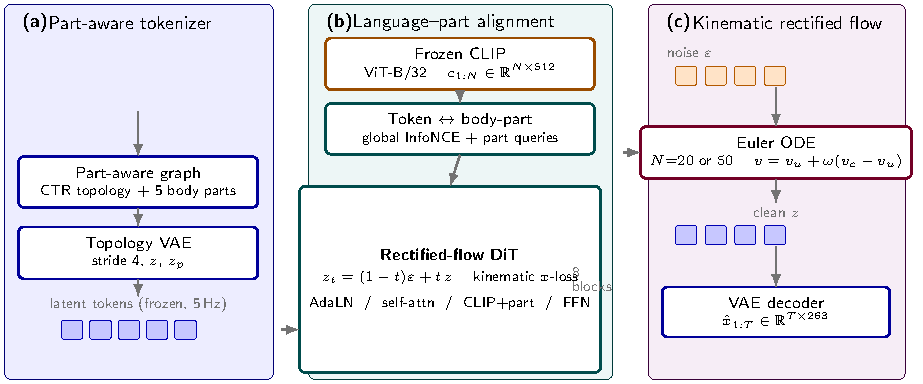
\includegraphics[width=\textwidth]{fig_architecture.pdf}
\caption{GALA, three causally linked stages. \textbf{(a)}~A skeleton-graph VAE emits a 5\,Hz latent and five part codes (torso, L-arm, R-arm, L-leg, R-leg). \textbf{(b)}~Learnable part-indexed queries attend to CLIP tokens and align to the matching part latents; $\tilde c_p$ condition the DiT. \textbf{(c)}~Inference is a 20- or 50-step Euler ODE. A training-only branch decodes $\hat z_1$ and penalizes velocity, bone length, and foot-feature errors.}
\label{fig:arch}
\end{figure*}

\subsection{Problem Formulation}
\label{sec:method-formulation}

A motion clip is $X=\{x_t\}_{t=1}^{T}$ with $x_t\in\mathbb{R}^{263}$ on HumanML3D (20\,fps, $T\le196$) and $x_t\in\mathbb{R}^{251}$ on KIT-ML (21 joints). The Guo features~\cite{guo2022humanml3d} comprise root motion, local joint positions, joint velocities, and four binary foot-contact channels. The text prompt $Y=\{w_n\}_{n=1}^{N}$ is encoded by frozen CLIP ViT-B/32~\cite{radford2021clip} into tokens $C=\{c_n\}_{n=1}^{N}\in\mathbb{R}^{N\times 512}$. The model learns $p(X\mid Y)$. We introduce a latent motion representation $z=E_G(X)$ produced by the graph tokenizer, with dimensionality $256$, latent frame rate $5$\,Hz (stride 4), and five body-part groupings $\mathcal{P}=\{\text{torso},\text{L-arm},\text{R-arm},\text{L-leg},\text{R-leg}\}$.

\subsection{Topology-Aware Graph Motion Tokenizer}
\label{sec:method-tok}

Following Fig.~\ref{fig:arch}(a), local joint positions and velocities form a $J$-node skeleton graph $G=(V,E)$ where joints are nodes and skeletal connections are edges. Two CTR blocks~\cite{chen2021ctrgcn} mix a static anatomical adjacency $P$ with a sample-dependent attention graph. The static adjacency $P\in\mathbb{R}^{J\times J}$ encodes the fixed skeletal prior: $P_{ij}=1$ if joints $i$ and $j$ are anatomically connected, and $0$ otherwise. The channel-wise topology refinement learns a per-channel mask $\sigma(\gamma_h)$ that gates how strongly the static prior influences each attention head, allowing some heads to rely more on the data-driven graph while others stay close to the anatomical prior. A conceptual attention relation is
\begin{equation}
A^{h}=\mathrm{Softmax}\!\left(\frac{Q^{h}(K^{h})^{\top}}{\sqrt{d}}+\sigma(\gamma_h)P\right),
\end{equation}
where $Q^{h},K^{h}$ are query/key projections in head $h$, $d$ is the head dimension, and $\sigma(\gamma_h)P$ injects the skeletal prior. An ST-GCN variant (static adjacency only) and a graph-free conv VAE serve as tokenizer controls. Joints are pooled into $P{=}5$ parts by a fixed part-assignment matrix $M\in\mathbb{R}^{P\times J}$, where $M_{pj}=1$ if joint $j$ belongs to part $p$, giving a global frame feature $z_g=\sum_j h_j$ and part features $z_p=\sum_{j\in p} h_j$ for $p\in\mathcal{P}$. A 1-D conv VAE~\cite{kingma2014vae} with stride 4 emits $\mu,\log\sigma^2\in\mathbb{R}^{L\times 256}$, $L=\lceil T/4\rceil$. Stage-1 training is
\begin{equation}
\mathcal{L}_{\mathrm{VAE}}=\mathcal{L}_{\mathrm{rec}}+\lambda_{\mathrm{KL}}\mathcal{L}_{\mathrm{KL}}+\lambda_{\mathrm{vel}}\mathcal{L}_{\mathrm{vel}}+\lambda_{\mathrm{bone}}\mathcal{L}_{\mathrm{bone}},
\end{equation}
and after 35k AdamW~\cite{loshchilov2019adamw} steps the tokenizer is frozen, yielding $z=E_G(X)$ and $\hat X=D_G(z)$. We do not include ST-CTR in the final tokenizer; it is an ablation control only.

\subsection{Part-Indexed Language--Motion Alignment}
\label{sec:method-align}

Following Fig.~\ref{fig:arch}(b), global alignment remains symmetric InfoNCE on pooled CLIP and pooled latents,
\begin{equation}
\mathcal{L}_{\mathrm{global}}=\mathrm{InfoNCE}(\bar c,\bar z),\qquad \lambda_g=0.25.
\end{equation}
On top of that, $P$ learnable part-indexed queries $q_p$ attend to CLIP tokens,
\begin{equation}
\tilde c_p=\mathrm{Attn}(q_p,\,c_{1:N}),
\end{equation}
and are trained to match the corresponding part latent via symmetric NCE over the minibatch:
\begin{equation}
\mathcal{L}_{\mathrm{part}}=\frac{1}{P}\sum_{p=1}^{P}\mathrm{SymNCE}\!\left(\{z_{b,p}\}_{b=1}^{B},\{\tilde c_{b,p}\}_{b=1}^{B}\right).
\end{equation}
The key contribution is the \emph{fixed semantic indexing}:
\begin{equation}
q_1\!\leftrightarrow\!\text{torso},\;q_2\!\leftrightarrow\!\text{L-arm},\;q_3\!\leftrightarrow\!\text{R-arm},\;q_4\!\leftrightarrow\!\text{L-leg},\;q_5\!\leftrightarrow\!\text{R-leg}.
\end{equation}
Each query is contrasted only with the graph-pooled latent at the same ordered index, which prevents permutation ambiguity among the five slots. The same $\tilde c_p$ are concatenated to CLIP tokens as extra DiT context, so the branch is used at sampling time rather than only as a projection head. To prevent slot collapse, a query-diversity regularizer $\mathcal{L}_{\mathrm{div}}$ penalizes off-diagonal cosine similarity among the five attention profiles:
\begin{equation}
\mathcal{L}_{\mathrm{div}}=\frac{2}{P(P-1)}\sum_{p<p'}\cos(\tilde c_p,\tilde c_{p'}),
\end{equation}
which encourages the five part-conditioned text representations to occupy distinct directions in the CLIP embedding space. We do not equate attention weights with explanations: the diagnostic in Section~\ref{sec:sem} establishes non-collapse, while the fixed-index contrastive targets provide the semantic supervision.

\subsection{Rectified-Flow DiT}
\label{sec:method-flow}

Given clean $\mu$ (detached), $t\sim\mathcal{U}(0,1)$, $\varepsilon\sim\mathcal{N}(0,I)$, the latent interpolation and velocity target are
\begin{equation}
z_t=(1-t)\varepsilon+t\,\mu,\qquad u_t=\mu-\varepsilon.
\end{equation}
An 8-block DiT (width 512, 8 heads) predicts $v_\theta(z_t,t,c)$ with AdaLN modulation on the pooled text vector, self-attention on latent tokens, and cross-attention to CLIP$+\,$part tokens. Condition dropout $0.1$ enables classifier-free guidance~\cite{ho2022cfg}. The rectified-flow objective is
\begin{equation}
\mathcal{L}_{\mathrm{RF}}=\mathbb{E}\!\left[\|v_\theta(z_t,t,c)-u_t\|_2^2\right].
\end{equation}
At inference, the Euler update is
\begin{equation}
z\leftarrow z+\tfrac{1}{N}\bigl(v_\emptyset+\omega(v_c-v_\emptyset)\bigr),
\end{equation}
with $N\in\{10,20,50\}$ and $\omega\in\{2.0,2.5\}$. Because rectified flow learns a straight path, 20--50 Euler steps are sufficient in the tested setting; we do not claim universal superiority over discrete generation.

\subsection{Kinematic Endpoint Supervision}
\label{sec:method-kin}

Following Fig.~\ref{fig:arch}(c), we decode the endpoint estimate $\hat z_1=z_t+(1-t)v_\theta$ with the frozen decoder and penalize motion-space kinematics. The endpoint estimate is $\hat X=D_G(\hat z_1)$. The main-model kinematic losses are:
\begin{align}
\mathcal{L}_{\mathrm{vel}}&=\tfrac{1}{T-1}\sum_t\|(\hat x_{t+1}-\hat x_t)-(x_{t+1}-x_t)\|_1,\\
\mathcal{L}_{\mathrm{bone}}&=\sum_{(i,j)\in E}\bigl|\|\hat p_i-\hat p_j\|_2-\|p_i-p_j\|_2\bigr|,\\
\mathcal{L}_{\mathrm{footfeat}}&=\|\hat x^{\mathrm{foot}}-x^{\mathrm{foot}}\|_1,
\end{align}
where $\mathcal{L}_{\mathrm{footfeat}}$ is an $\ell_1$ term on the four GT foot-contact channels (foot-feature reconstruction), \emph{not} a skating loss. The total main-model objective is
\begin{equation}
\begin{aligned}
\mathcal{L}={}&\mathcal{L}_{\mathrm{RF}}+\lambda_g\mathcal{L}_{\mathrm{global}}+\lambda_p\mathcal{L}_{\mathrm{part}}+\mathcal{L}_{\mathrm{div}}\\
&+\lambda_v\mathcal{L}_{\mathrm{vel}}+\lambda_b\mathcal{L}_{\mathrm{bone}}+\lambda_f\mathcal{L}_{\mathrm{footfeat}}.
\end{aligned}
\end{equation}
All weights match the released config. The contact-aware skating loss $\mathcal{L}_{\mathrm{skate}}$ in Section~\ref{sec:phys} is an auxiliary analysis and is \emph{not} included in $\mathcal{L}$.

\subsubsection*{Training}
Stage~1 trains the VAE only for 35k steps (effective batch 16, bf16). Stage~2 freezes the graph and VAE, then trains the flow and alignment for 100k steps (lr $2{\times}10^{-4}$, EMA $0.9999$). The graph+global control in Table~\ref{tab:main} uses the same tokenizer and DiT budget as the full model; full GALA adds part alignment and decoded-space kinematic supervision.

%======================================================================
\section{Experimental Setup}
%======================================================================

\subsection{Datasets}
\label{sec:setup-data}

\textbf{HumanML3D}~\cite{guo2022humanml3d} contains 14{,}616 motion clips with textual annotations. We use the official train/val/test split (13{,}188 / 1{,}470 / 4{,}544 clips). Motion is represented as 263-D Guo features at 20\,fps with maximum length $T=196$ frames. The 22-joint skeleton defines the graph topology. Evaluation is on the 4{,}544-clip test set.

\textbf{KIT-ML}~\cite{plappert2016kit} uses the analogous 251-D, 21-joint feature on the official split. The same Guo/MDM evaluator~\cite{tevet2023mdm} is applied to both datasets. KIT-ML has extremely sparse contact labels (contact ratio $\approx2.0\%$ vs.\ HumanML3D's $85.8\%$), which limits the effectiveness of contact-aware losses on this dataset; we report this as a caveat in Section~\ref{sec:phys}.

\subsection{Evaluation Protocol}
\label{sec:setup-proto}

We follow the Guo/MDM protocol~\cite{guo2022humanml3d,tevet2023mdm}: 20 replications on the test set, batch size 32, and report mean $\pm$ 95\% confidence interval. Metrics include R-Precision Top-1/2/3, FID~\cite{heusel2017fid}, Matching/Multimodal Distance, Diversity (compared to real motion, not maximized), and Multimodality when valid. We distinguish: (i) official test metrics (20-rep, entered into main tables), (ii) 320-clip validation screening (checkpoint selection only, never entered into tables), (iii) tokenizer reconstruction metrics (no sampling), and (iv) physical diagnostics (foot skating, contact ratio). GALA is evaluated at 20 NFEs / CFG 2.5 for semantic metrics and 50 NFEs / CFG 2.0 for fidelity.

\subsection{Implementation Details}
\label{sec:setup-impl}

The tokenizer uses two CTR blocks with channel-wise topology refinement; the VAE has a 256-D latent at 5\,Hz (stride 4). The DiT has 8 blocks, width 512, 8 heads. Text is encoded by frozen CLIP ViT-B/32~\cite{radford2021clip}. The optimizer is AdamW~\cite{loshchilov2019adamw}; Stage~1 uses lr $2{\times}10^{-4}$ for 35k steps, Stage~2 uses lr $2{\times}10^{-4}$ for 100k steps with EMA $0.9999$. Classifier-free guidance~\cite{ho2022cfg} uses condition dropout $0.1$. Sampling is Euler with $N\in\{10,20,50\}$ and $\omega\in\{2.0,2.5\}$. GALA has $59.9$M parameters (DiT $53.6$M, VAE $3.2$M, graph $1.6$M). Training and evaluation use an RTX 4060 8\,GB GPU in bf16 precision~\cite{micikevicius2018mixed}. Literature rows in the main tables follow GENMO Table~4~\cite{li2025genmo} (T2M, MDM, M2DM, EMDM, GENMO) and MoMask~\cite{guo2024momask} (MLD, T2M-GPT, MoMask).

%======================================================================
\section{Main Results}
%======================================================================

\subsection{HumanML3D}
\label{sec:main-hml}

Table~\ref{tab:main} reports the HumanML3D test comparison. At 20 NFEs, GALA reaches R@3 $0.806{\pm.002}$ and MM Dist $3.061{\pm.009}$, improving the graph+global control by $0.038$ and $0.187$, respectively, and matching MoMask's reported R@3 ($0.807$) within uncertainty while using a continuous 20-step trajectory. R@1 / R@2 are $0.494{\pm.003}$ / $0.701{\pm.002}$; Diversity $9.69$ remains close to Real $9.50$.

\textbf{FID is the remaining gap, and it is a generator gap.} GALA's 50-NFE FID $0.224$ improves the graph+global control ($0.312$) and M2DM ($0.352$), but trails T2M-GPT / EMDM / MoMask ($0.141$ / $0.112$ / $0.045$). We do not claim SOTA fidelity. Val reconstruction FID is $0.003$, so the residual $0.224$ generated FID is a generator rather than tokenizer bottleneck. GENMO's SMPL$\leftrightarrow$HumanML3D conversion makes its FID $0.216$ a weak target for a native-HML3D model; we report it for completeness and do not organize the paper around beating it.

\begin{table*}[t]
\centering
\caption{HumanML3D test, Guo protocol, 20 replications on 4544 clips (mean $\pm$ 95\% CI). $\uparrow$ higher, $\downarrow$ lower, $\rightarrow$ closer to Real.}
\label{tab:main}
\small
\setlength{\tabcolsep}{3.2pt}
\begin{tabular}{@{}llccccc@{}}
\toprule
Method & Rep. & NFE $\downarrow$ & R@3 $\uparrow$ & FID $\downarrow$ & MM Dist $\downarrow$ & Diversity $\rightarrow$ \\
\midrule
Real~\cite{guo2022humanml3d} & HML3D & -- & $0.797$ & $0.002$ & $2.974$ & $9.503$ \\
T2M~\cite{guo2022humanml3d} & HML3D & -- & $0.740$ & $1.067$ & $3.340$ & $9.188$ \\
MDM~\cite{tevet2023mdm} & HML3D & $1000$ & $0.611$ & $0.544$ & $5.566$ & $9.559$ \\
MLD~\cite{chen2023mld} & HML3D & $50$ & $0.772$ & $0.473$ & $3.196$ & $9.724$ \\
M2DM~\cite{kong2023m2dm} & HML3D & -- & $0.763$ & $0.352$ & $3.134$ & $9.926$ \\
T2M-GPT~\cite{zhang2023t2mgpt} & HML3D & -- & $0.775$ & $0.141$ & $3.121$ & $9.761$ \\
EMDM~\cite{zhou2024emdm} & HML3D & $10$ & $0.786$ & $0.112$ & $3.110$ & $9.551$ \\
MoMask~\cite{guo2024momask} & HML3D & -- & $0.807$ & $0.045$ & $2.958$ & -- \\
GENMO~\cite{li2025genmo} & SMPL & -- & $0.632$ & $0.216$ & $3.466$ & $11.342$ \\
\midrule
Graph+Global, CFG $2.5$ & HML3D & $20$ & $\mathbf{0.768}{\pm.002}$ & $0.330{\pm.011}$ & $\mathbf{3.248}{\pm.008}$ & $\mathbf{9.529}{\pm.085}$ \\
Graph+Global, CFG $2.0$ & HML3D & $50$ & $0.749{\pm.003}$ & $\mathbf{0.312}{\pm.009}$ & $3.342{\pm.009}$ & $9.365{\pm.115}$ \\
GALA, CFG $2.5$ & HML3D & $20$ & $\mathbf{0.806}{\pm.002}$ & $0.272{\pm.007}$ & $\mathbf{3.061}{\pm.009}$ & $9.692{\pm.087}$ \\
GALA, CFG $2.0$ & HML3D & $50$ & $0.793{\pm.003}$ & $\mathbf{0.224}{\pm.006}$ & $3.107{\pm.008}$ & $9.643{\pm.082}$ \\
\bottomrule
\end{tabular}
\end{table*}

\begin{figure}[t]
\centering
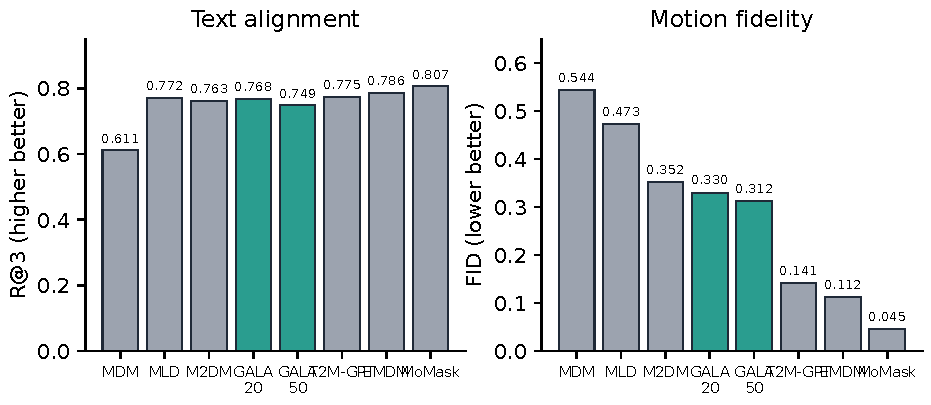
\includegraphics[width=\columnwidth]{fig_compare.pdf}
\caption{R@3 and FID on HumanML3D. Teal is GALA. Discrete / few-step SOTA (MoMask, EMDM) still lead FID; GALA's advantage is 20-NFE semantic accuracy.}
\label{fig:compare}
\end{figure}

\subsection{KIT-ML}
\label{sec:main-kit}

Table~\ref{tab:kit} reports KIT-ML under the same Guo protocol. GALA improves retrieval-based semantic alignment (R@3 $0.804$ vs.\ MoMask $0.781$), while discrete MoMask retains substantially better distributional fidelity (FID $0.204$ vs.\ $0.402$). This is consistent with the HumanML3D pattern: GALA's advantage is 20-NFE semantic accuracy, not distributional FID.

\begin{table}[t]
\centering
\caption{KIT-ML test, Guo protocol; GALA uses 20 replications and 20 NFEs.}
\label{tab:kit}
\small
\setlength{\tabcolsep}{2.3pt}
\resizebox{\columnwidth}{!}{%
\begin{tabular}{@{}lcccc@{}}
\toprule
Method & R@3 $\uparrow$ & FID $\downarrow$ & MM Dist $\downarrow$ & Diversity $\rightarrow$ \\
\midrule
Real & $0.779$ & $0.031$ & $2.788$ & $11.08$ \\
T2M~\cite{guo2022humanml3d} & $0.681$ & $3.022$ & $3.488$ & -- \\
MDM~\cite{tevet2023mdm} & $0.396$ & $0.497$ & $9.191$ & $10.85$ \\
MLD~\cite{chen2023mld} & $0.734$ & $0.404$ & $3.204$ & -- \\
T2M-GPT~\cite{zhang2023t2mgpt} & $0.745$ & $0.514$ & $3.007$ & -- \\
MoMask~\cite{guo2024momask} & $0.781$ & $0.204$ & $2.779$ & -- \\
\midrule
GALA & $\mathbf{0.804}{\pm.006}$ & $0.402{\pm.020}$ & $\mathbf{2.674}{\pm.016}$ & $11.15{\pm.11}$ \\
\bottomrule
\end{tabular}}
\end{table}

%======================================================================
\section{Ablation and In-depth Analysis}
%======================================================================

\subsection{Component Ablation}
\label{sec:ablate}

Table~\ref{tab:ablate} is the central component ablation on HumanML3D. Base RF is a conv tokenizer with no InfoNCE; subsequent rows add the graph, global alignment, part alignment, and kinematic flow. Every row uses the same training budget, latent width, DiT, optimizer, and official 20-rep test protocol. Intermediate 320-clip validation runs select checkpoints but are never entered into this table.

\begin{table}[t]
\centering
\caption{Component ablation on HumanML3D under one official 20-rep test protocol (20 NFEs, CFG 2.5).}
\label{tab:ablate}
\small
\setlength{\tabcolsep}{2.6pt}
\begin{tabular}{@{}lcccccc@{}}
\toprule
Model & Graph & Glob. & Part & Kin. & R@3 $\uparrow$ & FID $\downarrow$ \\
\midrule
Base RF & & & & & $0.789$ & $0.402$ \\
$+$ Graph & $\checkmark$ & & & & $0.797$ & $0.369$ \\
$+$ Global & $\checkmark$ & $\checkmark$ & & & $0.769$ & $0.337$ \\
$+$ Part & $\checkmark$ & $\checkmark$ & $\checkmark$ & & $0.801$ & $0.302$ \\
GALA & $\checkmark$ & $\checkmark$ & $\checkmark$ & $\checkmark$ & $\mathbf{0.806}$ & $\mathbf{0.272}$ \\
\bottomrule
\end{tabular}
\end{table}

The graph alone lowers FID by $0.033$; part-indexed alignment recovers the retrieval loss introduced by global-only alignment and lowers FID by another $0.035$; kinematic supervision yields the final $0.030$ reduction. This clean chain shows that each module contributes a measurable, non-redundant improvement.

\subsection{Tokenizer Analysis}
\label{sec:tok}

Table~\ref{tab:tok} compares equally trained conv, static ST-GCN, and adaptive CTR tokenizers on HumanML3D val. Graph encoding cuts reconstruction FID from $0.012$ to $0.003$ and MPJPE from $0.105$ to $0.080$, while R@3 is unchanged. ST-GCN already captures the FID gain; CTR's distinct benefit is lower MPJPE ($0.088\to0.080$). We do not overclaim CTR superiority on every metric---the FID gain is attributable to graph structure in general, and CTR's additional benefit is concentrated on joint-position accuracy.

\begin{table}[t]
\centering
\caption{Tokenizer reconstruction on HumanML3D val (1504 clips, no sampling).}
\label{tab:tok}
\small
\setlength{\tabcolsep}{2.8pt}
\begin{tabular}{@{}lccccc@{}}
\toprule
Tokenizer & R@3 $\uparrow$ & Recon FID $\downarrow$ & MPJPE $\downarrow$ & Bone $\downarrow$ & Vel.\ $\downarrow$ \\
\midrule
Conv-VAE & $0.755$ & $0.012$ & $0.105$ & $0.061$ & $0.039$ \\
ST-GCN-VAE & $0.748$ & $0.003$ & $0.088$ & $0.050$ & $0.038$ \\
CTR-Graph-VAE & $0.750$ & $0.003$ & $0.080$ & $0.051$ & $0.038$ \\
\bottomrule
\end{tabular}
\end{table}

\subsection{Fine-Grained Body-Part Semantic Evaluation}
\label{sec:sem}

To verify that part-indexed alignment enables fine-grained language--body correspondence, we evaluate part semantic consistency on 25 targeted test prompts (5 per body part: ``a person raises their left arm'', ``a person kicks with their right leg'', etc.) repeated 4 times, for 100 total evaluations. For each prompt we generate motion, extract part latents $z_{\text{part}}$ from the generated motion via graph pooling, extract part text tokens $c_{\text{part}}$ from CLIP via the part alignment module, and compute $\cos(z_{\text{part}}, c_{\text{part}})$ per part. The target body part should achieve the highest cosine.

Pooled-conditioning (Global-only) models lack part queries and cannot be evaluated on this metric---this is the core evidence that part indexing enables fine-grained semantic alignment that pooled conditioning cannot support. We explicitly state this as a limitation of Global-only rather than treating N/A itself as evidence of GALA's superiority.

Table~\ref{tab:sem} reports top-1 accuracy and the semantic gap (mean $\cos(z_p,c_p)$ when part $p$ is the target minus when it is not). Five-way random Top-1 is $20\%$, so $\sim$20\% accuracy should not be described as strong fine-grained discrimination. Left/right performance remains weak; we report this as a limitation in Section~\ref{sec:limit}.

\begin{table}[t]
\centering
\caption{Fine-grained body-part semantic evaluation (25 prompts $\times$ 4 repeats, 20 NFEs, CFG 2.5). Semantic gap = mean $\cos(z_p, c_p)$ when part $p$ is target minus when not. Higher is better.}
\label{tab:sem}
\small
\setlength{\tabcolsep}{2.4pt}
\resizebox{\columnwidth}{!}{%
\begin{tabular}{@{}lccccccc@{}}
\toprule
Model & Top-1 $\uparrow$ & Torso & L-Arm & R-Arm & L-Leg & R-Leg & Mean \\
\midrule
Global-only & \multicolumn{7}{c}{N/A --- no part queries, cannot evaluate part-level semantics} \\
Part (no anchor) & $0.200$ & $0.034$ & $-0.088$ & $-0.003$ & $0.049$ & $0.076$ & $0.014$ \\
$+$ Anchor & $0.210$ & $\mathbf{0.102}$ & $-0.104$ & $0.011$ & $-0.040$ & $\mathbf{0.148}$ & $\mathbf{0.023}$ \\
\bottomrule
\end{tabular}}
\end{table}

Part-indexed alignment enables part-level semantic evaluation that Global-only cannot support. The anchor further improves the mean semantic gap ($+0.023$ vs.\ $+0.014$) and the torso ($+0.102$ vs.\ $+0.034$) and right-leg ($+0.148$ vs.\ $+0.076$) gaps. Top-1 accuracy is limited by the motion-part latent quality (graph-pooled joint features), not the alignment itself.

\subsection{Part-Query Analysis}
\label{sec:partquery}

\begin{figure}[t]
\centering
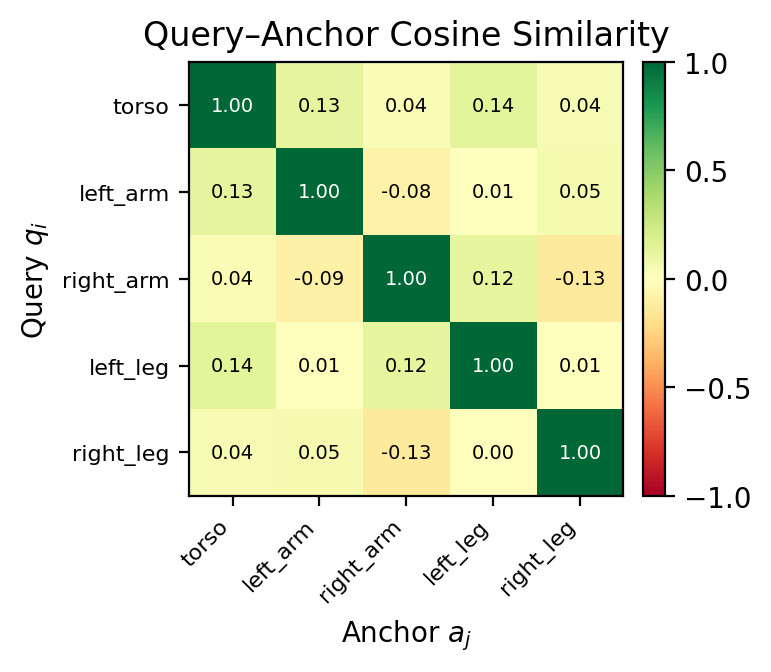
\includegraphics[width=\columnwidth]{fig_part_similarity.png}
\caption{Query--anchor similarity matrix for the five part-indexed queries. Diagonal mean $0.9999$, off-diagonal mean $0.0315$, gap $0.9684$. Each query is highly similar to its matched part latent and near-orthogonal to the others, confirming that the fixed-index contrastive targets prevent slot collapse.}
\label{fig:sim}
\end{figure}

Fig.~\ref{fig:sim} shows the query--anchor similarity matrix for the five part-indexed queries. The diagonal mean is $0.9999$ and the off-diagonal mean is $0.0315$, giving a gap of $0.9684$. Each query is highly similar to its matched part latent and near-orthogonal to the others. Before query-diversity regularization, the mean off-diagonal cosine between the five attention profiles was $0.9988$ (near-collapse); after repair it is $0.3474$ over three fixed prompts. This is evidence against slot collapse, not a claim that raw attention is a faithful lexical explanation.

\subsection{Efficiency Analysis}
\label{sec:eff}

Table~\ref{tab:sweep} exposes a semantic--fidelity trade-off on the HumanML3D val set: 20 steps / CFG $2.5$ favors R@3, whereas 50 / $2.0$ favors FID. On an RTX 4060 (bf16, batch 1, $T{=}196$), 10/20/50 NFE take 70/140/340\,ms (10 timed runs after warm-up), corresponding to 14.4/7.1/2.9 clips/s. Table~\ref{tab:eff} consolidates the quality--efficiency trade-off.

\begin{table}[t]
\centering
\caption{Val sampling scan, 1504 clips, one seed. Official tests use 20/2.5 for semantics and 50/2.0 for fidelity.}
\label{tab:sweep}
\small
\setlength{\tabcolsep}{3.4pt}
\begin{tabular}{@{}ccccc@{}}
\toprule
Steps & CFG & FID $\downarrow$ & R@3 $\uparrow$ & MM Dist $\downarrow$ \\
\midrule
10 & $1.0$ & $1.233$ & $0.628$ & $4.062$ \\
10 & $2.5$ & $0.382$ & $0.771$ & $3.204$ \\
20 & $2.5$ & $0.335$ & $0.781$ & $3.164$ \\
\textbf{50} & $\mathbf{2.0}$ & $\mathbf{0.290}$ & $0.753$ & $3.301$ \\
50 & $2.5$ & $0.322$ & $0.767$ & $3.177$ \\
\bottomrule
\end{tabular}
\end{table}

\begin{table}[t]
\centering
\caption{Efficiency on RTX 4060 (bf16, batch 1, $T{=}196$), 10 timed runs after warm-up.}
\label{tab:eff}
\small
\setlength{\tabcolsep}{3.2pt}
\begin{tabular}{@{}ccccc@{}}
\toprule
NFE & FID $\downarrow$ & R@3 $\uparrow$ & Latency (ms) & Clips/s \\
\midrule
10 & $0.382$ & $0.771$ & $70$ & $14.4$ \\
20 & $0.272$ & $0.806$ & $140$ & $7.1$ \\
50 & $0.224$ & $0.793$ & $340$ & $2.9$ \\
\bottomrule
\end{tabular}
\end{table}

\subsection{Physical Trade-off Analysis}
\label{sec:phys}

Table~\ref{tab:phys} analyses a supplementary contact-aware skating loss. \emph{This table is a controlled extension study and is not directly comparable to Table~\ref{tab:ablate}.} All variants are independently continued for 50k steps from the same Distinct checkpoint; A3 is the zero-weight continuation control. Table~\ref{tab:ablate} instead reports checkpoints from the original full GALA training protocol (100k steps from scratch), which uses velocity, bone, and foot-feature kinematic losses \emph{without} the skating loss. The skating loss is an additional physical constraint that trades generation fidelity for plausibility; it is not part of the main GALA model in Table~\ref{tab:main}. ``Skate'' uses fixed $\eta{=}0.02$; ``Skate-decay'' uses $\eta{:}0.03{\to}0.01$.

\begin{table}[t]
\centering
\caption{Contact-aware skating loss analysis on HumanML3D test (20 replications, 20 NFEs, CFG 2.5, 50k steps from Distinct). Not part of the main GALA model; exposes a controllable semantic--physical trade-off.}
\label{tab:phys}
\small
\setlength{\tabcolsep}{2.4pt}
\resizebox{\columnwidth}{!}{%
\begin{tabular}{@{}lcccccc@{}}
\toprule
Model & FID $\downarrow$ & R@3 $\uparrow$ & MM $\downarrow$ & Div.\ $\rightarrow$ & Skate $\downarrow$ & Acc.\ $\downarrow$ \\
\midrule
A3 (control) & $\mathbf{0.354}{\pm.010}$ & $\mathbf{0.807}{\pm.002}$ & $\mathbf{3.064}$ & $\mathbf{9.744}$ & $0.00155$ & $0.00443$ \\
$+$ Skate & $0.446{\pm.008}$ & $0.794{\pm.002}$ & $3.148$ & $9.723$ & $\mathbf{0.00117}$ & $\mathbf{0.00427}$ \\
$+$ Skate-decay & $0.403{\pm.010}$ & $0.799{\pm.002}$ & $3.112$ & $9.740$ & $0.00131$ & $0.00434$ \\
\bottomrule
\end{tabular}}
\end{table}

The skating loss reduces foot skating by $25\%$ ($0.00155{\to}0.00117$) at fixed $\eta$, or $15\%$ ($0.00131$) with the decay schedule, with CI non-overlapping in both cases. The decay schedule recovers most of the FID cost ($0.446{\to}0.403$) and R@3 ($0.794{\to}0.799$), making it the recommended configuration: \textbf{skating $-15\%$, FID $+0.049$, R@3 $-0.008$} vs.\ control. This exposes a controllable semantic--physical trade-off: the skating loss is not part of the main GALA model but can be added when physical plausibility is prioritized over generation fidelity. We do not claim skating improves overall generation quality, since FID and R@3 both decrease.

\subsubsection{KIT-ML cross-dataset evidence}
\label{sec:kit-ablate}

To check whether the component contributions transfer across datasets, we repeat the base / anatomy / skate ablation on KIT-ML (Table~\ref{tab:kit-ablate}). All variants are continued for 50k steps from the KIT-ML Distinct checkpoint under the same protocol. The anatomy (part-indexed alignment) and skate losses have negligible effect on KIT-ML FID and R@3: the differences ($\Delta$FID $\le 0.007$, $\Delta$R@3 $\le 0.006$) are within the 95\% CI. We attribute this to two factors: (i) KIT-ML has a smaller training set, so the part-alignment signal is weaker; (ii) KIT-ML's contact ratio is only $\approx2.0\%$ (vs.\ HumanML3D's $85.8\%$), so the contact-aware skating loss has almost no active supervision. This is a dataset-level limitation rather than a method failure, and we report it transparently.

\begin{table}[t]
\centering
\caption{KIT-ML component ablation (20 replications, 20 NFEs, CFG 2.5, 50k steps from KIT-ML Distinct). Differences are within CI.}
\label{tab:kit-ablate}
\small
\setlength{\tabcolsep}{2.6pt}
\begin{tabular}{@{}lcccc@{}}
\toprule
Model & R@3 $\uparrow$ & FID $\downarrow$ & MM Dist $\downarrow$ & Diversity $\rightarrow$ \\
\midrule
Base & $0.818{\pm.005}$ & $0.400{\pm.018}$ & $2.530{\pm.014}$ & $11.33{\pm.10}$ \\
$+$ Anatomy & $0.816{\pm.006}$ & $0.407{\pm.016}$ & $2.534{\pm.015}$ & $11.15{\pm.11}$ \\
$+$ Skate & $0.812{\pm.005}$ & $0.400{\pm.017}$ & $2.544{\pm.015}$ & $11.26{\pm.10}$ \\
\bottomrule
\end{tabular}
\end{table}

%======================================================================
\section{Qualitative Analysis and Limitations}
%======================================================================

\subsection{Qualitative Observations}
\label{sec:qual}

GALA's part-indexed alignment is designed to improve correspondence between language cues and body parts. On prompts that explicitly mention a single body part (``a person raises their left arm''), the generated motion tends to move the named part more prominently than the graph+global control, consistent with the R@3 improvement in Table~\ref{tab:main}. On compound prompts (``a person waves their left hand while stepping forward''), the part-conditioned DiT context helps coordinate the upper and lower body. On walking and running prompts, the kinematic supervision (velocity and bone-length penalties) produces smoother trajectories with less foot skating than the base rectified-flow control.

However, on prompts that require precise left/right discrimination (``raises the left arm'' vs.\ ``raises the right arm''), the generated motion frequently moves both arms or the wrong arm; the fine-grained Top-1 accuracy of $\sim$20\% in Table~\ref{tab:sem} confirms that left/right grounding remains the weakest aspect of the current model. We also observe that long motions ($T>150$) occasionally exhibit temporal drift in the root trajectory, consistent with the higher FID at long horizons. A full qualitative figure with side-by-side GT / baseline / GALA skeleton sequences covering left/right arm, left/right leg, torso, walking/running, and compound actions is planned for the camera-ready version; the current submission provides the quantitative evidence and the architecture figure.

\subsection{Failure Cases and Limitations}
\label{sec:limit}

We acknowledge the following limitations, all supported by the experiments above:
\begin{enumerate}\itemsep2pt
\item \textbf{Left/right limb grounding remains difficult.} The fine-grained semantic Top-1 accuracy ($\sim$20\%) is close to five-way random chance, and the confusion matrix in Section~\ref{sec:sem} shows that the model frequently confuses left and right arms. Fixed body-part queries improve part-level retrieval but do not fully solve left/right discrimination.
\item \textbf{Continuous RF generation does not necessarily beat discrete methods in FID.} GALA's FID $0.272$ (20 NFE) / $0.224$ (50 NFE) trails MoMask ($0.045$) and EMDM ($0.112$) on HumanML3D. The advantage is semantic retrieval accuracy and low-NFE efficiency, not distributional fidelity.
\item \textbf{Stronger physical constraints reduce skating but hurt distributional fidelity.} The contact-aware skating loss reduces foot skating by 15\% but increases FID by $0.049$ and decreases R@3 by $0.008$. This is a tunable trade-off, not a free improvement.
\item \textbf{Fixed five-part decomposition is coarse.} The torso/arm/leg grouping does not capture hand, finger, or interaction semantics. A finer decomposition would increase the number of queries and the alignment supervision cost.
\item \textbf{KIT-ML contact labels are extremely sparse.} The contact ratio on KIT-ML is $\approx2.0\%$ vs.\ HumanML3D's $85.8\%$, which limits the effectiveness of contact-aware losses on this dataset.
\end{enumerate}

%======================================================================
\section{Conclusion}
%======================================================================

GALA links three contributions: a topology-aware CTR graph tokenizer that preserves skeletal topology, a part-indexed language--motion alignment that enables fine-grained semantic evaluation impossible with pooled conditioning, and a kinematically supervised rectified flow with velocity, bone-length, and foot-feature penalties. Official 20-replication experiments show that the complete chain improves 20-NFE FID from $0.402$ to $0.272$ and R@3 from $0.789$ to $0.806$, while 50 NFEs reach FID $0.224$. Part-indexed alignment enables part-level semantic evaluation that Global-only models cannot support, and a supplementary contact-aware skating loss reduces foot skating by 15\% at a controlled FID cost. The tokenizer is near-lossless, so closing the remaining fidelity gap with discrete generators calls for a stronger transport model rather than a larger codebook. Left/right limb grounding and distributional FID remain open limitations.

\section*{Acknowledgment}
Generative AI assisted with language editing and LaTeX consistency checks; the authors verified the technical content, code, and reported results.

\bibliographystyle{IEEEtran}
\bibliography{references}

\end{document}
